\section*{2. Tiền xử lý dữ liệu}

\subsubsection*{Câu 2.1}

Cho thuộc tính ``tuổi'' với dãy giá trị đã sắp tăng dần ($n=27$):
\begin{center}
\small
$\begin{aligned}
&13,15,16,16,19,20,20,21,22,22,25,25,25,25,30,33,33,\\
&35,35,35,35,36,40,45,46,52,70.
\end{aligned}$
\end{center}

\textbf{Yêu cầu.} (a) Tính trung bình, trung vị, mốt. (b) Tìm tứ phân vị $Q_1$, $Q_3$ (có thể xấp xỉ nếu cần). (c) Vẽ boxplot và nhận xét phân bố. (d) Rời rạc hóa bằng phương pháp \emph{chia đều tần số} với $k=4$.

\medskip
\textbf{(a) Trung bình, trung vị, mốt.}

Tổng các giá trị bằng $809$, nên trung bình mẫu
\[
\bar x=\frac{809}{27}\approx 29{,}96.
\]

Vì $n$ lẻ, trung vị là phần tử vị trí thứ $\frac{n+1}{2}=14$ trên dãy đã sắp, đó là $25$.

Đếm tần số: $25$ và $35$ mỗi giá trị xuất hiện $4$ lần; các giá trị khác không quá $2$ lần. Vậy có hai mốt: $25$ và $35$ (đa mốt).

\textbf{(b) Tứ phân vị $Q_1$, $Q_3$.}

Có hai quy ước phổ biến; đề cho phép xấp xỉ.

\emph{Cách vị trí nguyên (1-based):} $Q_1$ ứng vị trí $\frac{1}{4}(n+1)=7$ $\Rightarrow$ giá trị thứ $7$ là $20$. $Q_3$ ứng vị trí $\frac{3}{4}(n+1)=21$ $\Rightarrow$ giá trị thứ $21$ là $35$. Khi đó $\mathrm{IQR}=35-20=15$.

\emph{Cách nội suy tuyến tính giữa hai quan sát kề:} vị trí $Q_1$ là $7{,}5$ nên $Q_1=\frac{20+21}{2}=20{,}5$; vị trí $Q_3$ là $20{,}5$ nên $Q_3=\frac{35+35}{2}=35$ và $\mathrm{IQR}=14{,}5$.

\textbf{(c) Boxplot và nhận xét.}

Năm số tóm tắt: $\min=13$, trung vị $=25$, $\max=70$; $Q_1,Q_3$ có thể lấy theo một trong hai cách ở (b). Ở đây minh họa với phép nội suy tuyến tính: $Q_1=20{,}5$, $Q_3=35$, $\mathrm{IQR}=14{,}5$. Ngưỡng trên Tukey là $Q_3+1{,}5\cdot\mathrm{IQR}=56{,}75$; vì $70>56{,}75$ nên $70$ thường được xem là ngoại lai phía trên. Trung bình ($\approx29{,}96$) lớn hơn trung vị ($25$) --- phân bố \emph{lệch phải} (đuôi dài về giá trị lớn).

\begin{center}
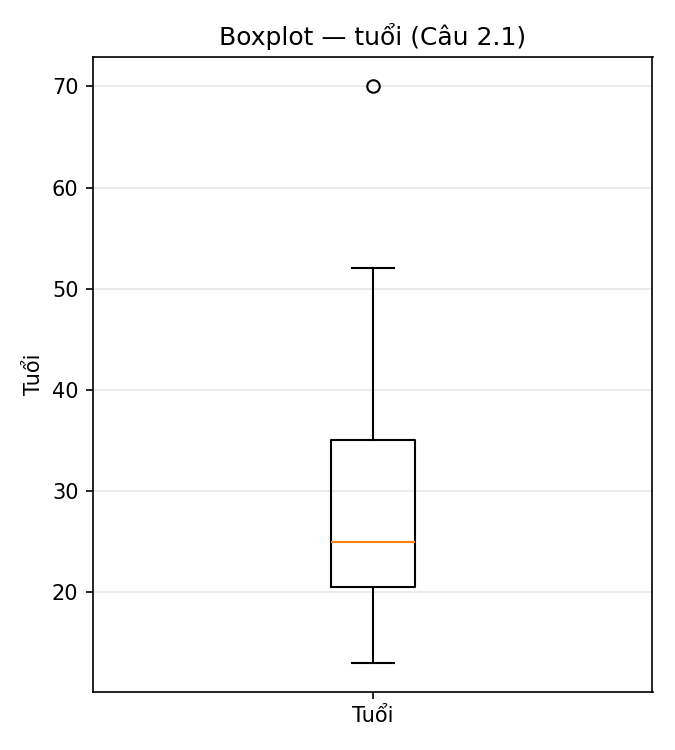
\includegraphics[width=0.55\textwidth]{figures/boxplot_tuoi.png}
\end{center}
\textit{Hình:} boxplot thuộc tính tuổi; râu và đánh dấu ngoại lai theo quy ước khoảng tứ phân vị và hệ số $1{,}5$ thông dụng.

\textbf{(d) Rời rạc hóa theo chia đều tần số, $k=4$.}

Với $n=27$, chia làm $4$ nhóm có số phần tử gần bằng nhau được $7{+}7{+}7{+}6$ phần tử nếu lấy $7$, $7$, $7$ phần tử nhỏ nhất rồi $6$ phần tử còn lại theo đúng thứ tự đã sắp:

\begin{itemize}
  \item Nhóm 1 ($7$ giá trị): từ $13$ đến $20$ --- $\{13,15,16,16,19,20,20\}$.
  \item Nhóm 2 ($7$ giá trị): từ $21$ đến $25$ --- $\{21,22,22,25,25,25,25\}$.
  \item Nhóm 3 ($7$ giá trị): từ $30$ đến $35$ --- $\{30,33,33,35,35,35,35\}$.
  \item Nhóm 4 ($6$ giá trị): từ $36$ đến $70$ --- $\{36,40,45,46,52,70\}$.
\end{itemize}

Cách gán nhãn lớp (ví dụ $B_1,\ldots,B_4$) có thể theo các khoảng trên cực độ tuổi trong từng nhóm; miễn là mọi điểm trong cùng một nhóm được gán \emph{một} lớp rời rạc và tần số các lớp gần bằng nhau như trên.

\emph{Chú ý so với chia độ rộng đều:} nếu chia $[\min,\max]$ thành bốn khoảng cùng độ rộng thì các lớp sẽ không còn tần số đều (thường dùng khi đề yêu cầu \emph{chia đều độ rộng}). Ở câu này đề chọn chia đều \emph{tần số}.

\subsubsection*{Câu 2.2}

Cho bảng giá trị sau trên các cột $A,B,C,D,E$:

\begin{center}
\small
\begin{tabular}{rccccc}
\toprule
Biến & $A$ & $B$ & $C$ & $D$ & $E$ \\\midrule
$V(\cdot)$    & $1$ & $2$ & $3$ & $4$ & $5$ \\
$W_1(\cdot)$  & $100$ & $200$ & $300$ & $400$ & $500$ \\
$W_2(\cdot)$  & $10$ & $11$ & $12$ & $13$ & $14$ \\
$W_3(\cdot)$  & $8$ & $13$ & $45$ & $6$ & $7$ \\
$W_4(\cdot)$  & $1$ & $4$ & $9$ & $16$ & $25$ \\
$W_5(\cdot)$  & $-10$ & $-8$ & $-6$ & $-4$ & $-2$ \\
$W_6(\cdot)$  & $3$ & $6$ & $9$ & $12$ & $15$ \\
\bottomrule
\end{tabular}
\end{center}

\textbf{Yêu cầu.} (1) Xác định thang đo của các giá trị $V$: (1) định danh, (2) thứ tự, (3) khoảng, (4) tỷ lệ. (2) Những biến $W_1,\ldots,W_6$ nào có cùng ``thông tin thang đo'' với $V(\cdot)$ trong nghĩa thang \emph{khoảng}.

\medskip
\textbf{(1) Thang đo của $V$.}

Các mức $1,\ldots,5$ có thứ tự rõ và khoảng cách giữa hai mức liền kề đều là $1$, nên \emph{hiệu} giữa hai giá trị có ý nghĩa (thang khoảng). Ngược lại không có căn cứ vật lý để coi một mức nào đó là ``không'' tuyệt đối của đại lượng theo nghĩa tỷ lệ (và tỷ số hai mức chưa hẳn diễn đạt ``gấp bao nhiêu lần'' trong thực tế). Do đó chọn loại $(3)$ \emph{thang khoảng} (interval).

\textbf{(2) Cùng thang khoảng với $V$.}

Hai biểu diễn số cùng thang khoảng nếu tồn tại phép đổi thang affine tăng: $W=aV+b$ với $a>0$, đúng trên đủ năm cột $(A,\ldots,E)$.

\begin{itemize}
  \item $W_1=100V$: lấy $a=100$, $b=0$.
  \item $W_2=V+9$: $a=1$, $b=9$.
  \item $W_3$: dãy giá trị $8,13,45,6,7$ không cùng thứ tự tăng với $V$; không có $a$, $b$ chung để $W_3=aV+b$ khớp năm cột --- \emph{không cùng}.
  \item $W_4=V^2$: khoảng tăng $W(4)-W(3)=16-9=7$ nhưng $W(3)-W(2)=9-4=5$ --- không đồng dạng một đường thẳng theo $V$ --- \emph{không cùng.}
  \item $W_5=2V-12$: $a=2$, $b=-12$.
  \item $W_6=3V$: $a=3$, $b=0$.
\end{itemize}

\textit{Kết luận:} các biểu diễn cùng thang khoảng với $V$: $W_1$, $W_2$, $W_5$, $W_6$; không cùng: $W_3$, $W_4$.
